\documentclass[aspectratio=169,10pt]{beamer}

% ==========================================================================
% THEME SETUP
% ==========================================================================

\usepackage{comment}

% Queen's University colors
\definecolor{QueensBlue}{HTML}{002452}
\definecolor{QueensRed}{HTML}{B90E31}
\definecolor{QueensGold}{HTML}{FABD0F}

\usetheme{default}
\setbeamertemplate{navigation symbols}{}
\setbeamertemplate{itemize items}{\textbullet}
\usefonttheme[onlymath]{serif}

% Colors
\setbeamercolor{frametitle}{fg=QueensRed}
\setbeamercolor{title}{fg=QueensGold}
\setbeamercolor{author}{fg=QueensGold}
\setbeamercolor{institute}{fg=QueensGold!80}
\setbeamercolor{date}{fg=QueensGold!80}
\setbeamercolor{structure}{fg=QueensBlue}
\setbeamercolor{block title}{fg=white, bg=QueensBlue}
\setbeamercolor{block body}{bg=QueensBlue!5}
\setbeamercolor{alerted text}{fg=QueensRed}
\setbeamercolor{section in head/foot}{fg=white, bg=QueensBlue}
\setbeamercolor{section in head/foot shaded}{fg=QueensBlue!40, bg=QueensBlue}

% Frame title
\setbeamerfont{frametitle}{size=\Large, series=\bfseries}
\setbeamertemplate{frametitle}{\vspace{0.3cm}\insertframetitle\par}

% Tri-color bar for normal frames (headline)
\setbeamertemplate{headline}{%
  \noindent\hbox to\paperwidth{%
    {\color{QueensBlue}\vrule height4pt width0.36\paperwidth}%
    {\color{QueensGold}\vrule height4pt width0.28\paperwidth}%
    {\color{QueensRed}\vrule height4pt width0.36\paperwidth}%
  }%
}


% Footline: section navigation
\setbeamertemplate{footline}{%
  \begin{beamercolorbox}[wd=\paperwidth, ht=2.5ex, dp=1.125ex]{section in head/foot}%
    \hfill\insertsectionnavigationhorizontal{0.95\paperwidth}{}{\hfill}\hfill%
  \end{beamercolorbox}%
}

% Section divider: colored background + centered white title
% Usage: \sectionslide{QueensRed}{Title Text}
\newcommand{\sectionslide}[2]{%
  \begingroup
  \setbeamercolor{background canvas}{bg=#1}
  \begin{frame}[plain,c]
    \centering{\Huge\bfseries\color{white}#2}
  \end{frame}
  \endgroup
}

% ==========================================================================
% PACKAGES
% ==========================================================================

\usepackage{amsmath,amssymb}
\PassOptionsToPackage{hyphens}{url}
\usepackage{hyperref}
\urlstyle{same}

% Footnote-style source citation pinned to bottom of slide
\newcommand{\source}[1]{\vfill{\tiny\color{gray}#1\par}}
\usepackage{booktabs}
\usepackage{graphicx}
\usepackage{tikz}
\usetikzlibrary{arrows.meta,positioning,calc,fit,backgrounds}

\graphicspath{{figures/}{../thesis/figures/}}

% ==========================================================================
% METADATA
% ==========================================================================

\title{Toward Visually Robust Quadruped Parkour\\via Monocular Depth Estimation}
\author{Theo Lemay\\[0.4em]{\small Supervisor: Prof.\ Joshua Marshall}}
\institute{Queen's University --- MTHE~499}
\date{April 2026}

\begin{document}

% ==========================================================================
% TITLE SLIDE
% ==========================================================================
{
\setbeamercolor{background canvas}{bg=QueensBlue}
\setbeamerfont{title}{size=\LARGE, series=\bfseries}
\setbeamercolor{title}{fg=white}
\begin{frame}[plain,c]
	\titlepage
\end{frame}
}
% SCRIPT: Good morning/afternoon. My name is Theo Lemay and I'm presenting my MTHE 499
% thesis. The title is "Toward Visually Robust Quadruped Parkour via Monocular Depth
% Estimation." I want to thank Prof. Marshall for supervising this project.


% ==========================================================================
\section{Background}
% ==========================================================================

\sectionslide{QueensRed}{Background}


% --- What is Quadruped Parkour? -------------------------------------------

\begin{frame}{What is Quadruped Parkour?}
\begin{columns}[T]
\column{0.52\textwidth}
  \begin{itemize}
    \setlength\itemsep{0.7em}
    \item \textbf{Quadruped robots} have four legs and can traverse unstructured terrain
    \item \textbf{Parkour}: traversing discrete structured obstacles ---
          stairs, hurdles, and gaps
    \item Policies are trained in \textbf{simulation via RL} and transferred to hardware
    \item Control runs at \textbf{50\,Hz}; perception must keep up
    \item Key challenge: the robot must \emph{perceive geometry} and
          \emph{coordinate} that with motor commands in real time
  \end{itemize}
\column{0.44\textwidth}
  % PLACEHOLDER: photo or video still of a real quadruped (Go2 or ANYmal)
  % mid-parkour over an obstacle. Suggested source: Extreme Parkour paper
  % (Cheng et al. 2023) or ANYmal Parkour (Hoeller et al. 2024) project page.
  \fbox{\parbox[c][5.5cm][c]{\linewidth}{\centering\color{gray}
    \textit{[PLACEHOLDER]}\\[0.4em]
    Photo/still: real quadruped\\
    doing parkour (Go2 or ANYmal)}}
\end{columns}
% SCRIPT: So first, what is quadruped parkour? We are talking about four-legged robots
% that need to cross discrete obstacles -- stairs, hurdles, and gaps -- in real time.
% Policies are trained in simulation using reinforcement learning and then transferred
% to the physical robot. The key challenge is that the robot needs to perceive the
% geometry of the obstacle in front of it, at 50 Hz, and coordinate that perception
% with 12 leg joints simultaneously.
\end{frame}


% --- Prior Work -----------------------------------------------------------

\begin{frame}{Prior Work: Learning to Parkour}
\begin{columns}[T]
\column{0.50\textwidth}
  {\small
  \begin{itemize}
    \setlength\itemsep{0.55em}
    \item \textbf{Legged Gym} \textcolor{gray}{\scriptsize[Rudin et al.\ 2022]} ---
          scalable sim-to-real RL framework; foundation of this work
    \item \textbf{Scandots} \textcolor{gray}{\scriptsize[Agarwal et al.\ 2023]} ---
          privileged teacher (heightmap) distilled into a depth-camera student
    \item \textbf{Extreme Parkour} \textcolor{gray}{\scriptsize[Cheng et al.\ 2023]} ---
          CNN--GRU student from depth; real-robot deployment
    \item \textbf{Robot Parkour Learning} \textcolor{gray}{\scriptsize[Zhuang et al.\ 2023]}
          --- multi-skill parkour on hardware
    \item \textbf{ANYmal Parkour} \textcolor{gray}{\scriptsize[Hoeller et al.\ 2024]} ---
          hierarchical skill selection
  \end{itemize}
  }
  \vspace{0.5em}
  \alert{All five systems assume a \textbf{depth camera} at deployment.}
\column{0.46\textwidth}
  % PLACEHOLDER: figure from the Extreme Parkour paper (Cheng et al. 2023)
  % showing the robot and obstacle course. Grab from their arXiv PDF or
  % project page at https://extreme-parkour.github.io
  \fbox{\parbox[c][5.5cm][c]{\linewidth}{\centering\color{gray}
    \textit{[PLACEHOLDER]}\\[0.4em]
    Figure from Extreme Parkour\\
    (Cheng et al.\ 2023)}}
\end{columns}
\source{Rudin et al.\ 2022 \textbar{} Agarwal et al.\ 2023 \textbar{}
        Cheng et al.\ 2023 \textbar{} Zhuang et al.\ 2023 \textbar{} Hoeller et al.\ 2024}
% SCRIPT: There has been significant progress in learning-based quadruped parkour. The
% Legged Gym framework made sim-to-real RL scalable. The Scandots paper introduced
% privileged teacher-student distillation. Extreme Parkour and Robot Parkour Learning
% deployed CNN-GRU policies on real robots. ANYmal Parkour added hierarchical skill
% selection. The common thread is that ALL of these systems use a dedicated depth
% camera at deployment. That's the assumption we are questioning.
\end{frame}


% --- Sim-to-Real ----------------------------------------------------------

\begin{frame}{Bridging Simulation to Reality: Three Strategies}
\begin{columns}[T]
\column{0.50\textwidth}
  \begin{enumerate}
    \setlength\itemsep{0.9em}
    \item \textbf{Domain Randomization} \textcolor{gray}{\scriptsize[Tobin et al.\ 2017]}\\
          Randomize textures and lighting at train time so the policy learns invariance

    \item \textbf{Generative Augmentation} \textcolor{gray}{\scriptsize[Yu et al.\ 2024
          --- LucidSim]}\\
          Replace synthetic frames with diffusion-rendered photorealistic images

    \item \textbf{Canonical Representation} $\leftarrow$ \emph{this work}\\
          Project both sim and real into a \textbf{shared depth space} via a
          pre-trained foundation model
  \end{enumerate}
\column{0.46\textwidth}
  % PLACEHOLDER: diagram showing sim RGB → DA2 → depth ← real RGB → DA2
  % as a "bridge" figure. Either a custom TikZ diagram or a screenshot
  % from the DA2 paper (Yang et al. 2024) showing real-world depth estimation.
  \fbox{\parbox[c][5.5cm][c]{\linewidth}{\centering\color{gray}
    \textit{[PLACEHOLDER]}\\[0.4em]
    Sim RGB / Real RGB $\xrightarrow{\text{DA2}}$ shared depth\\[0.3em]
    (custom diagram or DA2 demo figure)}}
\end{columns}
\source{Tobin et al.\ 2017 \textbar{} Yu et al.\ 2024 (LucidSim) \textbar{} Yang et al.\ 2024 (DA2)}
% SCRIPT: To deploy an RGB-only policy, you need to close the visual sim-to-real gap.
% Three strategies have emerged. Domain randomization randomizes appearances at train
% time. Generative augmentation uses diffusion models to produce photorealistic frames.
% This work takes a third approach: use a pre-trained depth estimator as a canonical
% representation, so both simulation and real images get projected into the same depth
% space -- without any domain randomization or photorealistic rendering.
\end{frame}


% --- Research Question ----------------------------------------------------

\begin{frame}{Research Question}
\begin{columns}[T]
\column{0.56\textwidth}
  \vspace{0.8em}
  \begin{block}{}
    \centering
    Can a pre-trained monocular depth estimator replace a depth camera
    and enable quadruped parkour from RGB --- without domain randomization?
  \end{block}

  \vspace{0.8em}
  \begin{itemize}
    \setlength\itemsep{0.6em}
    \item \textbf{Platform}: Unitree Go2 --- RGB camera only, no depth sensor
    \item \textbf{Estimator}: Depth Anything V2 (DA2) ---
          ViT trained on 142\,M diverse images
    \item \textbf{Scope}: simulation study; real-world transfer is future work
  \end{itemize}
\column{0.40\textwidth}
  % PLACEHOLDER: photo of the Unitree Go2 robot.
  % Source: https://www.unitree.com/go2/ or product press kit.
  \fbox{\parbox[c][5.5cm][c]{\linewidth}{\centering\color{gray}
    \textit{[PLACEHOLDER]}\\[0.4em]
    Unitree Go2 photo}}
\end{columns}
% SCRIPT: Our research question is: can a pre-trained monocular depth estimator replace
% a depth camera for quadruped parkour, without domain randomization? We target the
% Unitree Go2, which ships with only an RGB camera. We use Depth Anything V2 as the
% estimator -- it's a vision transformer trained on 142 million images. We evaluate
% entirely in simulation; real-world transfer is identified as future work.
\end{frame}


% ==========================================================================
\section{Math}
% ==========================================================================

\sectionslide{QueensRed}{Mathematical Framework}


% --- POMDP ----------------------------------------------------------------

\begin{frame}{Problem Formulation: POMDP}
\begin{columns}[T]
\column{0.50\textwidth}
  \textbf{Partially Observable MDP:}
  \[
    \bigl(\mathcal{S},\;\mathcal{A},\;\mathcal{O},\;T,\;R,\;Z\bigr)
  \]
  \begin{itemize}
    \setlength\itemsep{0.5em}
    \item \textbf{Action} $a \in \mathbb{R}^{12}$: joint position offsets,
          executed via PD controller at 50\,Hz
    \item Agent observes $o\!\in\!\mathcal{O}$, \emph{not} full state $s\!\in\!\mathcal{S}$
    \item Terrain geometry is \textbf{hidden} --- motivates privileged training and
          recurrent student architecture
  \end{itemize}

\column{0.46\textwidth}
  \vspace{0.3em}
  \textbf{Observation spaces:}\\[0.5em]
  {\small
  \begin{tabular}{@{}lrl@{}}
    \toprule
    Component & Dim & Content \\
    \midrule
    Proprioception & 53 & IMU, joints, cmds \\
    Teacher extero. & 132 & Scandot heightmap \\
    Student extero. & $58{\times}87$ & Depth image \\
    \bottomrule
  \end{tabular}
  }
  \vspace{0.8em}

  Partial observability $\Rightarrow$ \textbf{GRU} in student
  to approximate belief state
\end{columns}
% SCRIPT: The locomotion task is naturally formulated as a POMDP. The action space is
% 12-dimensional -- one joint offset per motor -- executed via a PD controller at 50 Hz.
% Crucially, the agent cannot directly observe the terrain geometry in front of it.
% The teacher gets around this with a privileged scandot heightmap. The student must
% infer terrain from a depth image. The partial observability is also why the student
% uses a GRU -- it can integrate information across time steps to approximate a belief
% state over the hidden terrain.
\end{frame}


% --- PPO ------------------------------------------------------------------

\begin{frame}{Teacher Training: Proximal Policy Optimization}
\begin{columns}[T]
\column{0.55\textwidth}
  \textbf{PPO clipped objective:}
  {\small
  \[
    \mathcal{L}^{\text{CLIP}} = \mathbb{E}_t\!\left[
      \min\!\Bigl(
        r_t\,\hat{A}_t,\;
        \operatorname{clip}(r_t,\,1{-}\varepsilon,\,1{+}\varepsilon)\,\hat{A}_t
      \Bigr)
    \right]
  \]
  }
  where $r_t = \pi_\theta(a_t|o_t)\,/\,\pi_{\theta_\text{old}}(a_t|o_t)$

  \vspace{0.6em}
  \begin{itemize}
    \setlength\itemsep{0.5em}
    \item Clipping keeps the policy update in a \textbf{trust region}
    \item \textbf{GAE} advantage estimate: $\hat{A}_t$ balances
          bias ($\lambda{\to}0$) vs.\ variance ($\lambda{\to}1$)
    \item Teacher has \textbf{full access} to scandot heightmap ---
          achieves $\approx99\%$ success across all difficulties
  \end{itemize}

\column{0.40\textwidth}
  % Optional: teacher_training.pdf shows training reward curve.
  % Either include it here or use a PLACEHOLDER for a clean diagram
  % showing the teacher architecture with scandots input.
  % PLACEHOLDER: diagram of teacher MLP with scandot heightmap input,
  % or include 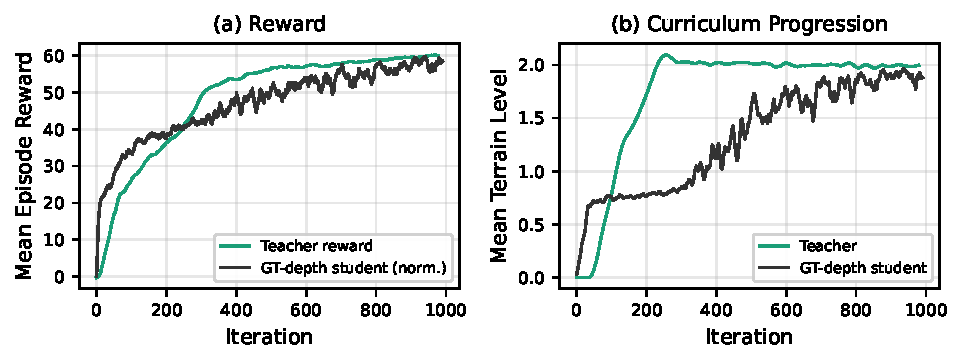
\includegraphics[width=\linewidth]{teacher_training.pdf}
  \fbox{\parbox[c][5cm][c]{\linewidth}{\centering\color{gray}
    \textit{[PLACEHOLDER]}\\[0.4em]
    Teacher architecture diagram\\
    or training reward curve\\
    (\texttt{teacher\_training.pdf})}}
\end{columns}
% SCRIPT: The teacher is trained with PPO. The clipped objective prevents the policy
% from taking steps that are too large -- it restricts the probability ratio between
% new and old policy to stay in the interval 1-epsilon to 1+epsilon. Advantage is
% estimated via GAE, which lets you tune the bias-variance tradeoff with lambda.
% The teacher has full access to a scandot heightmap -- ground-truth terrain geometry
% from laser scans -- so it can achieve near-perfect performance.
\end{frame}


% --- DAgger ---------------------------------------------------------------

\begin{frame}{Student Distillation: DAgger}
\begin{columns}[T]
\column{0.52\textwidth}
  \textbf{Why not behavioral cloning?}
  \begin{itemize}
    \item BC on a fixed dataset $\Rightarrow$ \textbf{error compounding}
    \item Student mistakes shift the state distribution --- it encounters
          states never seen in training $\Rightarrow$ policy collapse
  \end{itemize}

  \vspace{0.6em}
  \textbf{DAgger (Ross et al.\ 2011):}
  \begin{enumerate}
    \setlength\itemsep{0.3em}
    \item Roll out under \textbf{student policy}
    \item Label visited states with \textbf{teacher's actions}
    \item Aggregate into training set; retrain student
    \item Repeat
  \end{enumerate}

  \vspace{0.5em}
  Loss combines action imitation + yaw heading:
  \[ \mathcal{L} = \mathcal{L}_{\text{action}} + \mathcal{L}_{\text{yaw}} \]

\column{0.44\textwidth}
  % PLACEHOLDER: DAgger loop diagram.
  % Options: (1) figure from Ross et al. 2011 AISTATS paper,
  % (2) custom TikZ showing Student → env → Teacher label → dataset → Student loop.
  \fbox{\parbox[c][5.5cm][c]{\linewidth}{\centering\color{gray}
    \textit{[PLACEHOLDER]}\\[0.4em]
    DAgger loop diagram\\
    (custom TikZ or Ross et al.\ 2011)}}
\end{columns}
% SCRIPT: To train the student, we use DAgger -- Dataset Aggregation. Naive behavioral
% cloning on a fixed expert dataset fails because of error compounding: small mistakes
% put the student in states it never saw during training, and errors accumulate.
% DAgger fixes this by collecting rollouts under the STUDENT's own policy, then asking
% the teacher what the correct action would have been. This means the student's training
% distribution always matches its deployment distribution. The loss combines imitation
% of the teacher's joint targets with a yaw heading term to keep the robot oriented correctly.
\end{frame}


% ==========================================================================
\section{Architecture}
% ==========================================================================

\sectionslide{QueensRed}{System Architecture}


% --- Pipeline -------------------------------------------------------------

\begin{frame}{Two-Stage Teacher--Student Pipeline}
\vspace{-0.2cm}
\begin{center}
  \scalebox{0.88}{%
    % Pipeline diagram: two-stage teacher-student distillation
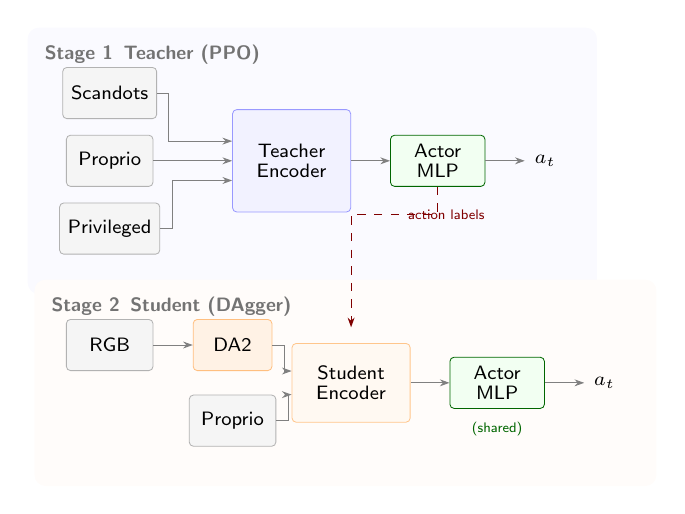
\begin{tikzpicture}[
  >=Stealth,
  % --- shared block base ---
  blkbase/.style={
    rounded corners=1.5pt, minimum height=6.5mm,
    inner xsep=3pt, inner ysep=1.5pt,
    line width=0.3pt, align=center, font=\scriptsize\sffamily
  },
  % --- block types ---
  inp/.style={blkbase, draw=black!30, fill=gray!8, minimum width=11mm},
  da2/.style={blkbase, draw=orange!50, fill=orange!10, minimum width=10mm},
  tenc/.style={blkbase, draw=blue!40, fill=blue!5, minimum width=15mm, minimum height=13mm},
  senc/.style={blkbase, draw=orange!45, fill=orange!5, minimum width=15mm, minimum height=10mm},
  act/.style={blkbase, draw=green!40!black, fill=green!5, minimum width=12mm},
  % --- labels ---
  outlbl/.style={font=\scriptsize\sffamily},
  stglbl/.style={font=\scriptsize\sffamily\bfseries, text=black!55, anchor=north west},
  annot/.style={font=\tiny\sffamily},
  % --- arrows ---
  arr/.style={-{Stealth[length=3.5pt, width=2.5pt]}, line width=0.35pt, draw=black!50},
  darr/.style={-{Stealth[length=3.5pt, width=2.5pt]}, line width=0.4pt, dashed, draw=red!50!black},
]

% ===================== STAGE 1: TEACHER =====================

\node[inp] (scan) at (0, 0) {Scandots};
\node[inp, below=2mm of scan] (prop1) {Proprio};
\node[inp, below=2mm of prop1] (priv) {Privileged};

\node[tenc, right=10mm of prop1] (te) {Teacher\\[-1pt]Encoder};
\node[act] (ta) at ([xshift=11mm]te.east) {Actor\\[-1pt]MLP};
\node[outlbl, right=5mm of ta] (tout) {$a_t$};

\draw[arr] (scan.east) -- ++(1.5mm,0) |- ([yshift=2.5mm]te.west);
\draw[arr] (prop1) -- (te);
\draw[arr] (priv.east) -- ++(1.5mm,0) |- ([yshift=-2.5mm]te.west);
\draw[arr] (te) -- (ta);
\draw[arr] (ta) -- (tout);

% Stage 1 background
\begin{scope}[on background layer]
  \node[draw=none, fill=blue!2, rounded corners=4pt,
    fit=(scan)(priv)(tout), inner xsep=4mm, inner ysep=5mm] (s1) {};
  \node[stglbl] at ([xshift=1mm, yshift=-1mm]s1.north west)
    {Stage 1\enspace Teacher (PPO)};
\end{scope}

% ===================== STAGE 2: STUDENT =====================

\node[inp] (rgb) at (0, -3.2) {RGB};
\node[da2, right=5mm of rgb] (d2) {DA2};
\node[inp, below=3mm of d2] (prop2) {Proprio};

\node[senc] (se) at ([xshift=10mm]d2.east |- {$(d2)!0.5!(prop2)$}) {Student\\[-1pt]Encoder};
\node[act] (sa) at ([xshift=11mm]se.east) {Actor\\[-1pt]MLP};
\node[outlbl, right=5mm of sa] (sout) {$a_t$};

\draw[arr] (rgb) -- (d2);
\draw[arr] (d2.east) -- ++(1.5mm,0) |- ([yshift=1.5mm]se.west);
\draw[arr] (prop2.east) -- ++(1.5mm,0) |- ([yshift=-1.5mm]se.west);
\draw[arr] (se) -- (sa);
\draw[arr] (sa) -- (sout);

% Stage 2 background
\begin{scope}[on background layer]
  \node[draw=none, fill=orange!2, rounded corners=4pt,
    fit=(rgb)(prop2)(sout), inner xsep=4mm, inner ysep=5mm] (s2) {};
  \node[stglbl] at ([xshift=1mm, yshift=-1mm]s2.north west)
    {Stage 2\enspace Student (DAgger)};
\end{scope}

% ===================== CONNECTIONS =====================

% DAgger supervision arrow
\draw[darr]
  (ta.south) -- ++(0,-3.5mm)
  -| node[pos=0.25, right=0.5mm, annot, text=red!50!black] {action labels}
  ([yshift=2mm]se.north);

% Shared actor annotation
\node[annot, text=green!40!black, below=0.5mm of sa] {(shared)};

\end{tikzpicture}
%
  }
\end{center}
\vspace{-0.3cm}
{\small
\textbf{Stage~1 (PPO):} Teacher trained with privileged scandot heightmap ---
near-perfect performance. \quad
\textbf{Stage~2 (DAgger):} Student learns to mimic teacher from DA2 estimated
depth images.
}
% SCRIPT: Here is the full two-stage pipeline. On the left, the teacher policy takes
% proprioception and the scandot heightmap, runs it through parallel MLPs to produce
% a terrain latent vector and an action. On the right, the student replaces the
% heightmap with a 58x87 depth image from Depth Anything V2, processes it through
% a CNN and GRU, and produces the same terrain latent to feed into the SAME frozen
% actor MLP as the teacher. DAgger trains the student's encoder by rolling out in
% the environment and using the teacher's actions as labels.
\end{frame}


% --- Student Architecture -------------------------------------------------

\begin{frame}{Student Architecture \& DSQ Metric}
\begin{columns}[T]
\column{0.48\textwidth}
  \textbf{Student visual encoder (CNN--GRU):}
  \vspace{0.2em}
  \begin{center}
    \scalebox{0.78}{%
      % Student visual encoder architecture
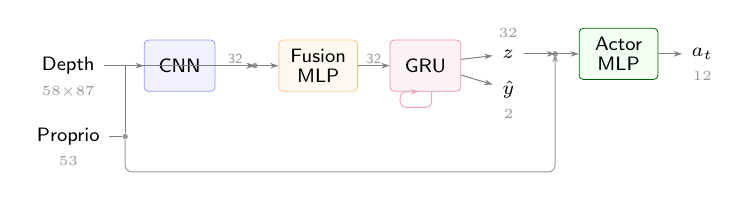
\begin{tikzpicture}[
  >=Stealth,
  % --- shared block base ---
  blkbase/.style={
    rounded corners=1.5pt, minimum height=6.5mm,
    inner xsep=2.5pt, inner ysep=1.5pt,
    line width=0.3pt, align=center, font=\scriptsize\sffamily
  },
  % --- block types ---
  cnn/.style={blkbase, draw=blue!40, fill=blue!5, minimum width=9mm},
  fuse/.style={blkbase, draw=orange!45, fill=orange!5, minimum width=10mm},
  gru/.style={blkbase, draw=purple!40, fill=purple!5, minimum width=9mm},
  act/.style={blkbase, draw=green!40!black, fill=green!5, minimum width=10mm},
  % --- labels ---
  io/.style={font=\scriptsize\sffamily},
  dim/.style={font=\tiny\sffamily, text=black!40, inner sep=0.5pt},
  % --- arrows ---
  arr/.style={-{Stealth[length=3pt, width=2pt]}, line width=0.35pt, draw=black!50},
]

% ===================== INPUTS =====================

\node[io] (depth) at (0, 0.4) {Depth};
\node[dim, below=0mm of depth] {$58{\times}87$};

\node[io] (prop) at (0, -0.5) {Proprio};
\node[dim, below=0mm of prop] {$53$};

% ===================== PROCESSING =====================

\node[cnn, right=5mm of depth] (cnn) {CNN};

% Concat point 1
\coordinate (cat1) at ([xshift=5mm]cnn.east);
\node[circle, fill=black!40, inner sep=0.7pt] at (cat1) {};

\node[fuse, right=3mm of cat1] (fmlp) {Fusion\\[-1pt]MLP};

\node[gru, right=4mm of fmlp] (gru) {GRU};

% GRU recurrence
\draw[arr, rounded corners=2pt, draw=purple!35]
  ([xshift=0.8mm]gru.south) -- ++(0,-2mm) -- ++(-4mm,0) -- ++(0,2mm)
  -- ([xshift=-0.8mm]gru.south);

% ===================== GRU OUTPUTS =====================

\node[io, right=4mm of gru, yshift=1.5mm] (z) {$z$};
\node[dim, above=0mm of z] {$32$};
\node[io, right=4mm of gru, yshift=-3mm] (yhat) {$\hat{y}$};
\node[dim, below=0mm of yhat] {$2$};

% Concat point 2
\coordinate (cat2) at ([xshift=4mm]z.east);
\node[circle, fill=black!40, inner sep=0.7pt] at (cat2) {};

\node[act, right=3mm of cat2] (actor) {Actor\\[-1pt]MLP};

\node[io, right=3mm of actor] (out) {$a_t$};
\node[dim, below=0mm of out] {$12$};

% ===================== ARROWS =====================

\draw[arr] (depth) -- (cnn);
\draw[arr] (cnn) -- node[dim, above] {32} (cat1);
\draw[arr] (cat1) -- (fmlp);
\draw[arr] (fmlp) -- node[dim, above] {32} (gru);
\draw[arr] ([yshift=0.8mm]gru.east) -- (z);
\draw[arr] ([yshift=-1.2mm]gru.east) -- (yhat);
\draw[arr] (z) -- (cat2);
\draw[arr] (cat2) -- (actor);
\draw[arr] (actor) -- (out);

% Proprio branch point
\node[circle, fill=black!40, inner sep=0.7pt] (pbr) at ([xshift=2mm]prop.east) {};

% Branch 1: to fusion
\draw[arr] (prop.east) -- (pbr) |- (cat1);

% Branch 2: to actor (route below)
\draw[arr, rounded corners=2.5pt, draw=black!40]
  (pbr) -- ++(0,-4.5mm) -| (cat2);

\end{tikzpicture}
%
    }
  \end{center}
  {\small
  \begin{itemize}
    \item $58{\times}87$ depth $\to$ CNN $\to$ 32-dim features
    \item GRU integrates temporally (belief state)
    \item Reuses teacher's frozen actor MLP
  \end{itemize}
  }

\column{0.48\textwidth}
  \textbf{Depth Signal Quality (DSQ):}
  \[
    \text{DSQ} = \frac{1}{T}\frac{1}{N}\sum_{t,i}
      \rho\!\left(d^{\text{GT}}_i,\, d^{\text{DA2}}_i\right)
  \]
  where $\rho$ is Pearson correlation.

  \vspace{0.5em}
  \begin{itemize}
    \setlength\itemsep{0.4em}
    \item \textbf{Affine-invariant} --- handles monocular scale-shift ambiguity
    \item Low DSQ $\Leftrightarrow$ degraded depth estimate $\Leftrightarrow$ policy fails
    \item Averaged over environments and time steps
  \end{itemize}
\end{columns}
% SCRIPT: The student's visual encoder is a CNN-GRU. The CNN processes a 58x87
% depth image -- small enough for fast inference -- into a 32-dimensional feature
% vector. That's concatenated with proprioception, fed through a GRU for temporal
% integration, and produces the terrain latent that the frozen actor MLP converts
% to joint targets. We also introduce DSQ -- Depth Signal Quality -- as a diagnostic
% metric. It's the Pearson correlation between ground-truth and DA2 estimated depth.
% Pearson correlation is affine-invariant, which is important because monocular depth
% estimators have an inherent scale-shift ambiguity -- they can't know the absolute
% scale. DSQ being low is a reliable indicator that the policy will fail.
\end{frame}


% ==========================================================================
\section{Results}
% ==========================================================================

\sectionslide{QueensRed}{Experiments \& Results}


% --- Baselines ------------------------------------------------------------

\begin{frame}{Baselines: Upper Bounds}
\begin{center}
{\small
\begin{tabular}{@{}lcccc@{}}
\toprule
 & Row~0 & Row~1 & Row~2 & Row~3 \\
 & \scriptsize(easy) & & & \scriptsize(hard) \\
\midrule
Scandots teacher   & 98.5 & 100.0 & 99.0 & 98.5 \\
GT-depth student   & 94.5 & 94.5  & 89.1 & 87.5 \\
Zero-depth ablation & 8.0 & 2.0   & 0.0  & 0.0  \\
\bottomrule
\end{tabular}
}
\end{center}

\vspace{0.6em}
\begin{itemize}
  \setlength\itemsep{0.5em}
  \item The CNN--GRU architecture \textbf{works from depth} ---
        GT-depth student $\approx$ teacher performance
  \item Zero-depth ablation confirms: policy relies on
        \textbf{depth, not proprioceptive heuristics} alone
  \item Question: can DA2 estimated depth close the remaining gap?
\end{itemize}

\vspace{0.3em}
{\small Success rate (\%) on gap terrain, averaged over 256 episodes.}
% SCRIPT: Before testing DA2, we establish baselines. The scandots teacher achieves
% near-perfect performance. The ground-truth depth student -- using the exact same
% depth image the simulator would produce from a real depth camera -- also performs
% well, 87 to 94 percent. This is our upper bound. The zero-depth ablation -- same
% architecture but black image -- drops to near zero. This confirms that the policy
% is actually using the depth signal, not just relying on proprioception to jump at
% the right time. The question is: can Depth Anything V2's estimates be good enough?
\end{frame}


% --- DA2 Results ----------------------------------------------------------

\begin{frame}{Model Scale \& Terrain Texture}
\begin{columns}[T]
\column{0.46\textwidth}
  {\small
  \begin{tabular}{@{}lcccc@{}}
  \toprule
  Configuration & R0 & R1 & R2 & R3 \\
  \midrule
  DA2-small          & 56.3 & 33.6 & ---  & ---  \\
  DA2-base           & 68.4 & 83.2 & 26.6 & 0.8  \\
  DA2-base + texture & 64.8 & 64.1 & 68.0 & 44.9 \\
  \midrule
  GT-depth (upper bound) & 94.5 & 94.5 & 89.1 & 87.5 \\
  \bottomrule
  \end{tabular}
  }
  \vspace{0.6em}
  \begin{itemize}
    \setlength\itemsep{0.4em}
    \item Larger model $\Rightarrow$ better depth $\Rightarrow$ higher success
    \item \textbf{Untextured terrain}: gap boundary is ambiguous to DA2
    \item Adding checkerboard \textbf{texture} recovers most of the gap
          to GT-depth on harder rows
  \end{itemize}

\column{0.50\textwidth}
  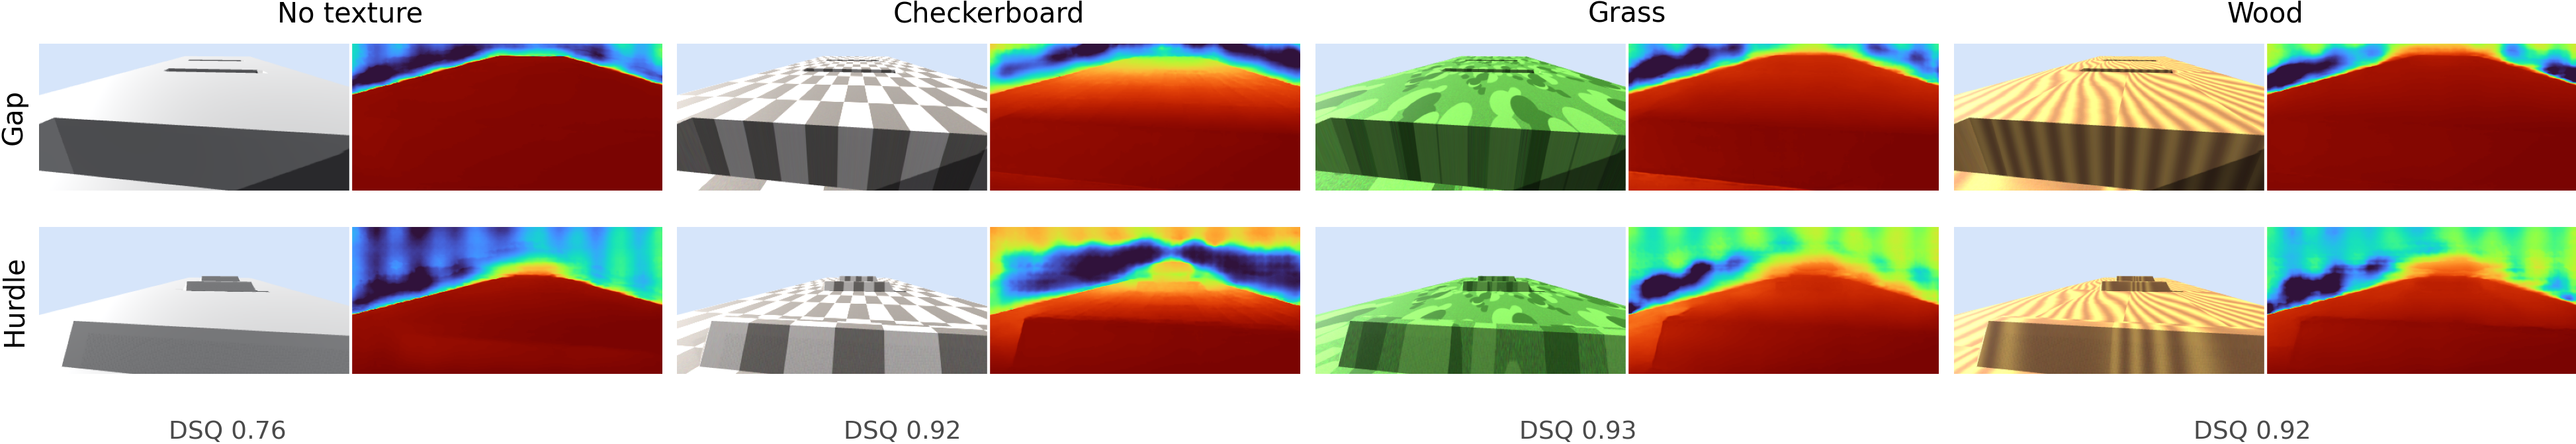
\includegraphics[width=\linewidth]{da2_texture_comparison.png}
  \vspace{0.2em}
  {\tiny Each panel: RGB (left) and DA2 depth estimate (right).
  Featureless terrain produces weakest obstacle localization.}
\end{columns}
% SCRIPT: Now we replace the ground-truth depth with DA2 estimates. DA2-small partially
% works but fails on the harder rows. DA2-base improves significantly on rows 0 and 1.
% But on untextured terrain, the gap boundary is ambiguous -- there's no texture gradient
% for DA2 to latch onto, so it produces flat, uninformative depth maps. When we add a
% checkerboard texture to the terrain, the gap geometry becomes visible, and performance
% on row 2 jumps from 26.6% to 68%. You can see this in the figure -- featureless terrain
% on the left produces flat depth; checkerboard on the right produces a clear step.
\end{frame}


% --- Visual Sensitivity ---------------------------------------------------

\begin{frame}{Visual Sensitivity Study}
\begin{columns}[T]
\column{0.46\textwidth}
  \textbf{Key findings across 6 terrain configurations:}
  \vspace{0.4em}
  \begin{itemize}
    \setlength\itemsep{0.45em}
    \item \textbf{Stairs \& hurdles}: robust to lighting and color
          shifts (strong edges persist across conditions)
    \item \textbf{Gaps}: always texture-sensitive --- boundary
          visible mainly through surface features
    \item \textbf{Featureless}: catastrophic failure
          ($96\% \to 17\%$ on gap Row~0; $0\%$ on Row~3)
    \item \textbf{Dim lighting} (0.3$\times$): moderate degradation only
    \item \textbf{Combined extreme}: $34\%$ on gap Row~0,
          $0.4\%$ on Row~3
    \item DSQ useful failure indicator --- but high DSQ alone
          does not guarantee robustness on unseen textures
  \end{itemize}

\column{0.50\textwidth}
  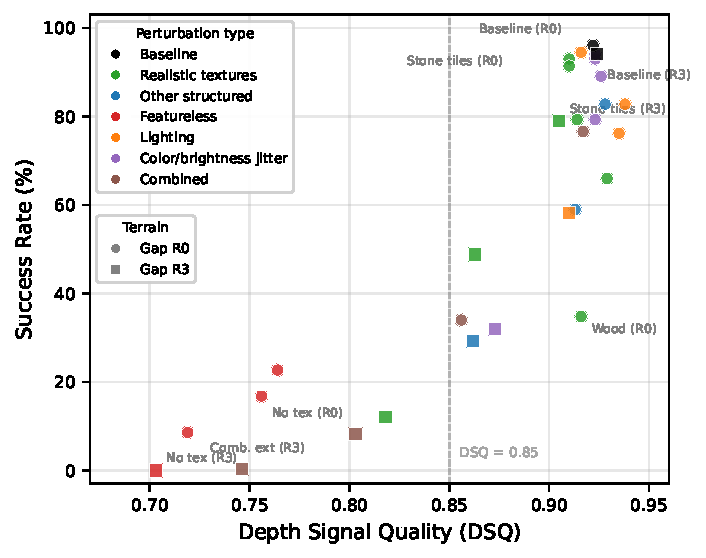
\includegraphics[width=\linewidth]{dsq_scatter.pdf}
  \vspace{0.2em}
  {\tiny Success rate vs.\ DSQ. Color = obstacle type/difficulty;
  shape = perturbation type.}
\end{columns}
% SCRIPT: We then perturbed the trained student at test time only -- no retraining.
% Stairs and hurdles are largely robust because their edges remain visible under
% most conditions. Gaps are the most texture-sensitive: the gap boundary is only
% visible as a texture discontinuity, so featureless terrain collapses success.
% Lighting changes alone cause only moderate degradation. The scatter plot shows
% DSQ versus success across all conditions. You can see a clear correlation --
% low DSQ predicts failure -- but the relationship isn't perfect: some unseen
% textures maintain high DSQ but still reduce performance, suggesting the policy
% has some sensitivity beyond just raw depth quality.
\end{frame}


% --- Discussion -----------------------------------------------------------

\begin{frame}{Discussion \& Limitations}
\begin{columns}[T]
\column{0.48\textwidth}
  \textbf{What we learned:}
  \begin{itemize}
    \setlength\itemsep{0.45em}
    \item Monocular depth is a \textbf{viable canonical representation}
          for sim-to-real parkour --- works in simulation
    \item Moderate robustness to photometric variation
          \textbf{without domain randomization}
    \item Bottleneck is \textbf{depth quality}, not student architecture
    \item Gap traversal the hardest case; texture is the key factor
  \end{itemize}

\column{0.48\textwidth}
  \textbf{Limitations \& future work:}
  \begin{itemize}
    \setlength\itemsep{0.45em}
    \item \alert{Simulation only} --- no hardware validation yet
    \item DA2-base too heavy for onboard inference
    \item Frame-independent estimation --- no temporal consistency
    \item DA2 fails on transparent surfaces, thin structures,
          close-range objects
    \item Next: real robot evaluation; joint depth\,+\,policy
          adaptation; temporally-aware estimators
  \end{itemize}
\end{columns}
% SCRIPT: To summarize: monocular depth is a viable approach for sim-based quadruped
% parkour. We get moderate photometric robustness for free, without any domain
% randomization. The main bottleneck is depth quality -- if DA2 can't see the obstacle
% boundary, the policy fails. The most important limitation is that we only validated
% in simulation. Real hardware would introduce motion blur, exposure shifts, and real
% depth scale ambiguity that we haven't tested. Future work would evaluate on a real Go2,
% and potentially co-adapt the depth estimator and the policy end-to-end.
\end{frame}


% ==========================================================================
% CLOSING
% ==========================================================================

\sectionslide{QueensBlue}{Thank you! \\[1em]Questions?}

\end{document}
